\documentclass[conference]{IEEEtran}
\IEEEoverridecommandlockouts

\usepackage{cite}
\usepackage{amsmath,amssymb,amsfonts}
\usepackage{algorithmic}
\usepackage{graphicx}
\usepackage{textcomp}
\usepackage{xcolor}
\usepackage{caption}
\usepackage{float}
\usepackage{graphicx}
\usepackage{hyperref}
\usepackage{float}


\def\BibTeX{{\rm B\kern-.05em{\sc i\kern-.025em b}\kern-.08em
    T\kern-.1667em\lower.7ex\hbox{E}\kern-.125emX}}

\title{Simulaci\'on y An\'alisis del Robot xArm6 en ROS 2 y Gazebo}

\author
{
\IEEEauthorblockN{Clarissa Gardea Coronado}
\IEEEauthorblockA{\textit{Estudiante de Robótica} \\
\textit{Tecnológico de Monterrey}\\
Zapopan, México \\
a01569420@tec.mx}
\and
\IEEEauthorblockN{Arturo Azael Godínez Rodríguez}
\IEEEauthorblockA{\textit{Estudiante de Robótica} \\
\textit{Tecnológico de Monterrey}\\
Zapopan, México \\
a01641179@tec.mx}
\and
\IEEEauthorblockN{David Gómez Carrillo}
\IEEEauthorblockA{\textit{Estudiante de Robótica} \\
\textit{Tecnológico de Monterrey}\\
Zapopan, México \\
a01642824@tec.mx}
\and
\IEEEauthorblockN{Andrés Lepe Alvarado}
\IEEEauthorblockA{\textit{Estudiante de Robótica} \\
\textit{Tecnológico de Monterrey}\\
Zapopan, México \\
a01643265@tec.mx}
\and
\IEEEauthorblockN{Christian Omar Payán Torróntegui}
\IEEEauthorblockA{\textit{Estudiante de Robótica} \\
\textit{Tecnológico de Monterrey}\\
Zapopan, México\\
a01742658@tec.mx}
\and
}

\begin{document}

\maketitle

\begin{abstract}
Este trabajo presenta la simulación, modelado y control del brazo robótico \textit{xArm6} utilizando el entorno robótico ROS 2. Se realizó un análisis cinemático mediante el método de Denavit-Hartenberg (DH) para describir la cadena cinemática del manipulador, cuyos resultados fueron validados visualmente en RViz mediante la publicación de un marcador en la posición del efector final. Además, se implementó la simulación del robot en Gazebo con el entorno \texttt{xarm\_gazebo}, configurando controladores con \texttt{ros2\_control} para ejecutar trayectorias articuladas. Finalmente, se diseñó e implementó una secuencia de movimientos tipo sentadilla como demostración de control personalizado, validando así la coherencia entre el modelo analítico, el descriptivo (URDF) y el comportamiento simulado.
\end{abstract}


\begin{IEEEkeywords}
xArm6, ROS 2, Gazebo, RViz, ROS Control, Cinemática inversa Denavit-Hartenberg, Control de trayectorias, URDF
\end{IEEEkeywords}

\section{Introducci\'on}

En este trabajo se llevó a cabo la simulación y control del brazo robótico xArm6 utilizando ROS 2. Se trabajó principalmente con los entornos de Gazebo y RViz para visualizar la configuración del robot y validar su funcionamiento. La simulación incluyó la activación de controladores, la ejecución de trayectorias y la representación del entorno con una mesa como obstáculo.

Como parte de la práctica, se configuraron los controladores necesarios mediante comandos de ROS 2 Control y se utilizó un nodo en Python para enviar una trayectoria específica que simula un movimiento de flexión del brazo. Esta trayectoria fue ejecutada correctamente en el simulador Gazebo, permitiendo observar la respuesta del robot ante comandos personalizados. Además, se comprobó la comunicación entre los distintos nodos y tópicos del sistema, asegurando que el robot respondiera adecuadamente a los mensajes de control.

\section{Análisis Cinemático: Tabla de Denavit-Hartenberg}

Con el objetivo de analizar el comportamiento cinemático del brazo robótico \textit{xArm6}, se ha utilizado el método de Denavit-Hartenberg (DH) para describir su cadena cinemática. Este método permite expresar cada transformación entre eslabones consecutivos mediante cuatro parámetros: el ángulo articular $\theta_i$, la distancia $d_i$, la longitud del eslabón $a_i$, y el ángulo de torsión $\alpha_i$.

La identificación de los parámetros DH se realizó a partir del modelo URDF del robot contenido en el paquete \texttt{xarm\_description}, en combinación con la documentación técnica proporcionada por UFactory. Se seleccionaron como marcos de referencia aquellos que cumplen con las convenciones clásicas de DH, ubicando el eje $z_i$ como el eje de giro de cada articulación y siguiendo la disposición mecánica del robot. La tabla resultante se presenta a continuación:

\begin{table}[H]
\centering
\caption{Parámetros DH del xArm6}
\begin{tabular}{|c|c|c|c|c|}
\hline
\textbf{Articulación $i$} & $\theta_i$ (rad) & $d_i$ (m) & $a_i$ (m) & $\alpha_i$ (rad) \\
\hline
1 & $\theta_1$ & 0.267 & 0     & $-\frac{\pi}{2}$ \\
2 & $\theta_2$ & 0     & 0.293 & $0$              \\
3 & $\theta_3$ & 0     & 0.300 & $0$              \\
4 & $\theta_4$ & 0.302 & 0     & $-\frac{\pi}{2}$ \\
5 & $\theta_5$ & 0     & 0     & $\frac{\pi}{2}$  \\
6 & $\theta_6$ & 0.072 & 0     & $0$              \\
\hline
\end{tabular}
\label{tab:dh_xarm6}
\end{table}

Los parámetros se definieron de la siguiente forma:
\begin{itemize}
    \item $\theta_i$: ángulo articular variable de cada articulación rotacional.
    \item $d_i$: desplazamiento a lo largo del eje $z_{i-1}$.
    \item $a_i$: longitud del eslabón, distancia entre ejes $z_{i-1}$ y $z_i$ medida sobre $x_{i-1}$.
    \item $\alpha_i$: ángulo entre ejes $z_{i-1}$ y $z_i$ alrededor de $x_{i-1}$.
\end{itemize}.

\subsubsection*{Formación de parámetros y de la cadena cinemática}

Los parámetros de la tabla DH fueron obtenidos a partir del modelo URDF oficial del xArm6, el cual describe las dimensiones geométricas y la disposición relativa de cada eslabón. Para cada articulación, se identificaron los ejes de rotación (ejes $z$) y las distancias entre ejes consecutivos, lo cual permitió asignar los valores de $d_i$, $a_i$ y $\alpha_i$ siguiendo las convenciones estándar de Denavit-Hartenberg. 

El ángulo $\theta_i$ se mantiene como variable, ya que cada articulación es de tipo rotacional. La secuencia de marcos de referencia fue construida asegurando que el eje $z_i$ coincida con el eje de rotación de la $i$-ésima articulación, y el eje $x_i$ apunte desde $z_{i-1}$ hacia $z_i$ de forma perpendicular. De esta manera, se forma una cadena cinemática en la que cada transformación homogénea representa el cambio de coordenadas entre eslabones consecutivos. Esta descripción fue validada comparando la posición del efector final resultante con la generada por el modelo URDF.


\section{Visualización de la Posición del Efector Final en RViz}

Para validar la cadena cinemática modelada mediante los parámetros de Denavit-Hartenberg, se eligió una configuración articular específica del robot \textit{xArm6} y se calculó manualmente la posición del efector final utilizando transformaciones homogéneas. Posteriormente, esta posición fue representada gráficamente en RViz mediante un mensaje de tipo \texttt{visualization\_msgs::Marker}.

La configuración articular utilizada fue:
\begin{equation}
\theta = [0^\circ,\ 0^\circ,\ 90^\circ,\ 0^\circ,\ 0^\circ,\ 0^\circ]
\end{equation}

A partir de la tabla DH y esta configuración, se construyeron las matrices homogéneas $A_i$ para cada articulación:
\[
A_i = 
\begin{bmatrix}
\cos\theta_i & -\sin\theta_i\cos\alpha_i & \sin\theta_i\sin\alpha_i & a_i\cos\theta_i \\
\sin\theta_i & \cos\theta_i\cos\alpha_i & -\cos\theta_i\sin\alpha_i & a_i\sin\theta_i \\
0 & \sin\alpha_i & \cos\alpha_i & d_i \\
0 & 0 & 0 & 1
\end{bmatrix}
\]

La transformación total se obtuvo mediante la multiplicación sucesiva:
\[
T_0^6 = A_1 A_2 A_3 A_4 A_5 A_6
\]

El vector de posición del efector final se extrae de la última columna de la matriz $T_0^6$.

\section{Visualización de la posición del efector final en RViz}

Para verificar la posición del efector final, se utilizó el paquete \texttt{robot\_state\_publisher} junto con \texttt{joint\_state\_publisher\_gui}, lo cual permitió manipular la configuración articular del robot de forma gráfica. 

A partir de dicha configuración, se publicó un marcador tipo esfera mediante un nodo en Python que consulta la transformada \texttt{link\_base $\rightarrow$ link\_eef} usando \texttt{tf2}. La posición del marcador coincide con la posición calculada del efector final, validando así que la cadena cinemática esté correctamente descrita en el modelo URDF.

\begin{figure}[H]
    \centering
    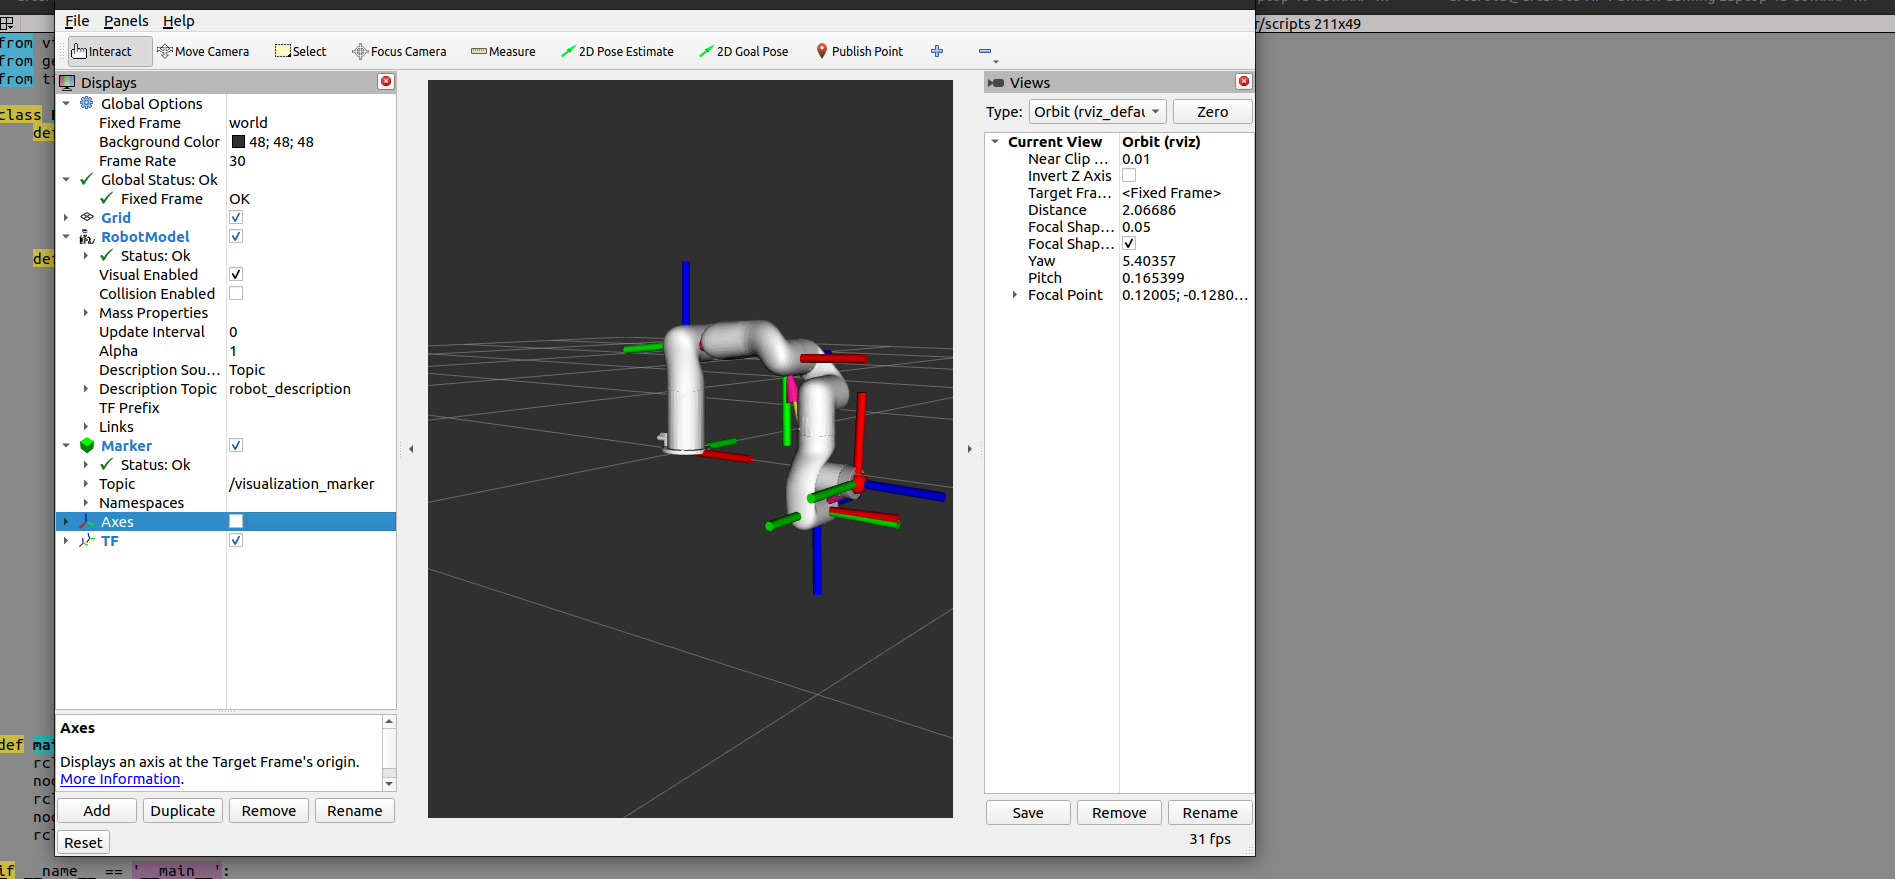
\includegraphics[width=0.47\textwidth]{images/robot_con_marker.png}
    \caption{Visualización del robot en RViz con el marcador del efector final (esfera roja).}
    \label{fig:rviz_marker}
\end{figure}

\begin{figure}[H]
    \centering
    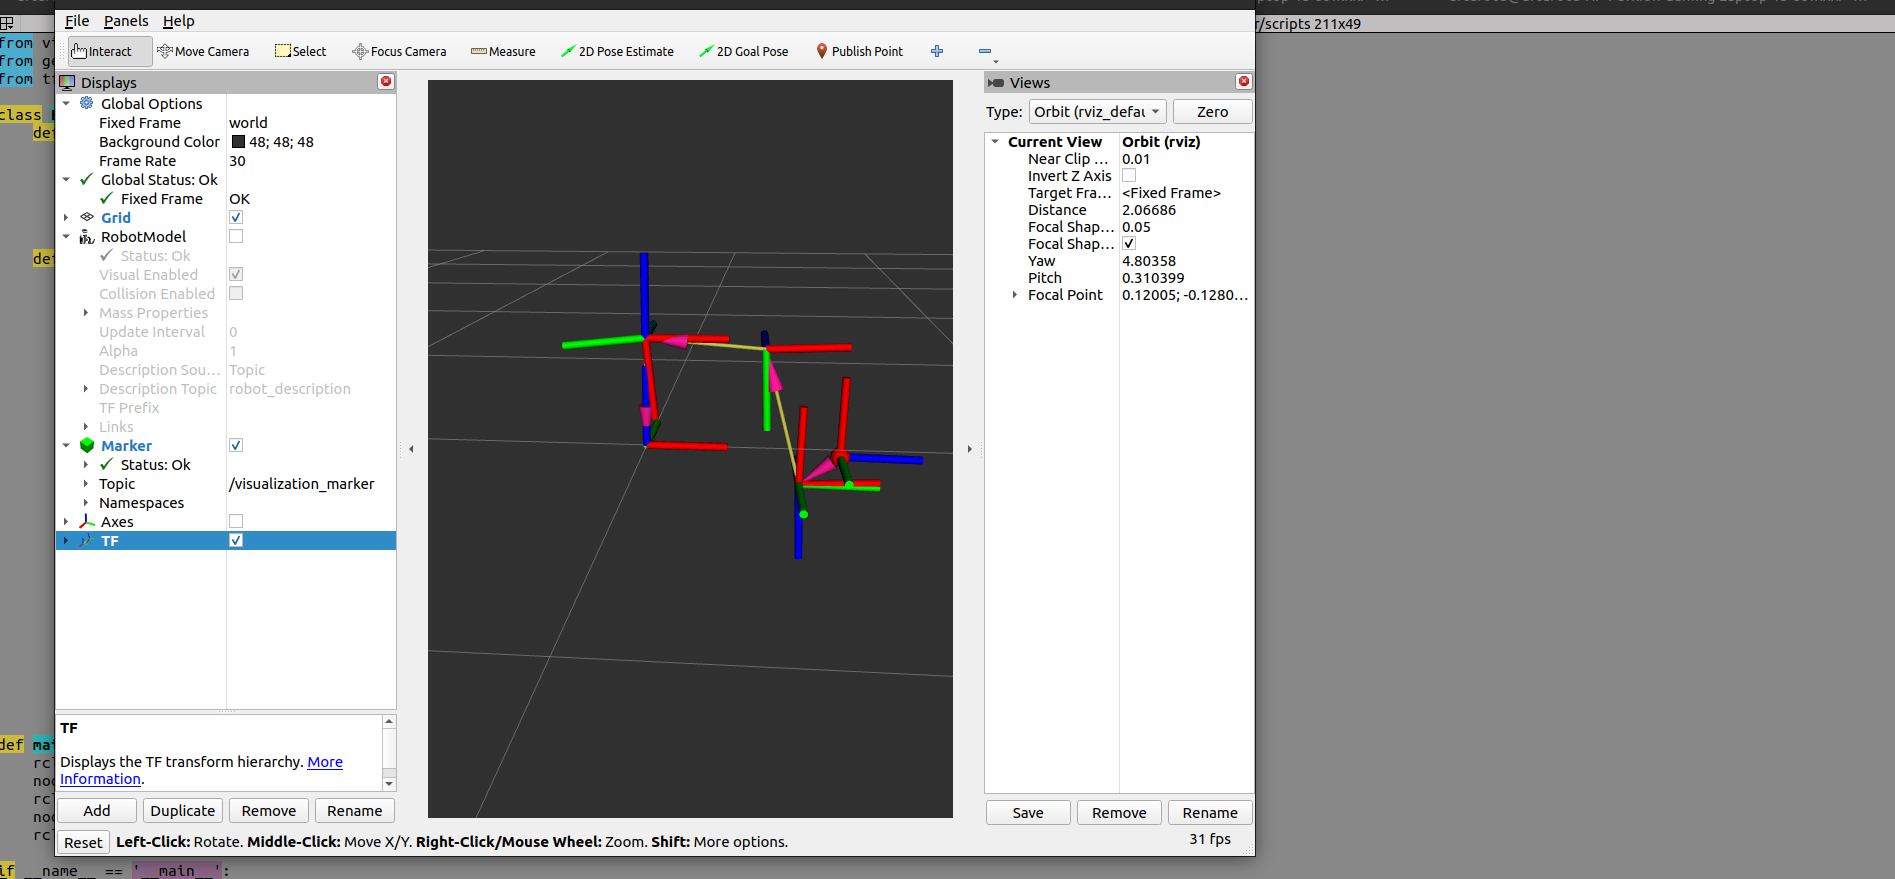
\includegraphics[width=0.47\textwidth]{images/sin_robot.png}
    \caption{Visualización de los marcos de referencia del robot. El marcador coincide con el frame del efector final.}
    \label{fig:rviz_tf}
\end{figure}







\subsubsection*{Verificación en RViz}

Para la visualización se lanzaron los nodos \texttt{robot\_state\_publisher} y \texttt{joint\_state\_publisher\_gui}, permitiendo modificar los ángulos articulares en tiempo real. Se comprobó que la posición del marcador coincidía visualmente con el \texttt{tf} del efector final publicado por el URDF, verificando así la consistencia entre el modelo analítico (DH) y el modelo descriptivo (URDF).


\section{Simulación en Gazebo con controladores}

Para validar el comportamiento del modelo cinemático en un entorno físico simulado, se utilizó el simulador Gazebo junto con el paquete \texttt{xarm\_gazebo}. El robot se posicionó sobre una mesa en un entorno controlado, lo cual permite recrear tareas colaborativas en un espacio limitado.

El modelo fue cargado mediante el siguiente comando:

\texttt{\detokenize{ros2 launch xarm_gazebo xarm6_beside_table_gazebo.launch.py}}

A continuación, se habilitó la interfaz de control usando los siguientes comandos desde terminal:

\begin{itemize}
    \item Activación del \texttt{joint\_state\_broadcaster}:\\
    \texttt{\detokenize{ros2 control load_controller --set-state active joint_state_broadcaster}}

    \item Activación del controlador principal de trayectoria:\\
    \texttt{\detokenize{ros2 control load_controller --set-state active xarm6_traj_controller}}
\end{itemize}

Una vez cargados los controladores, se verificó la disponibilidad del tópico de acción:
\begin{verbatim}
ros2 topic list | grep trajectory
\end{verbatim}

Esto permitió enviar comandos de movimiento al robot simulando el efecto de una flexión o postura inicial. La Figura~\ref{fig:gazebo_home} muestra la posición inicial del brazo sobre la mesa dentro del entorno de Gazebo.

\begin{figure}[H]
    \centering
    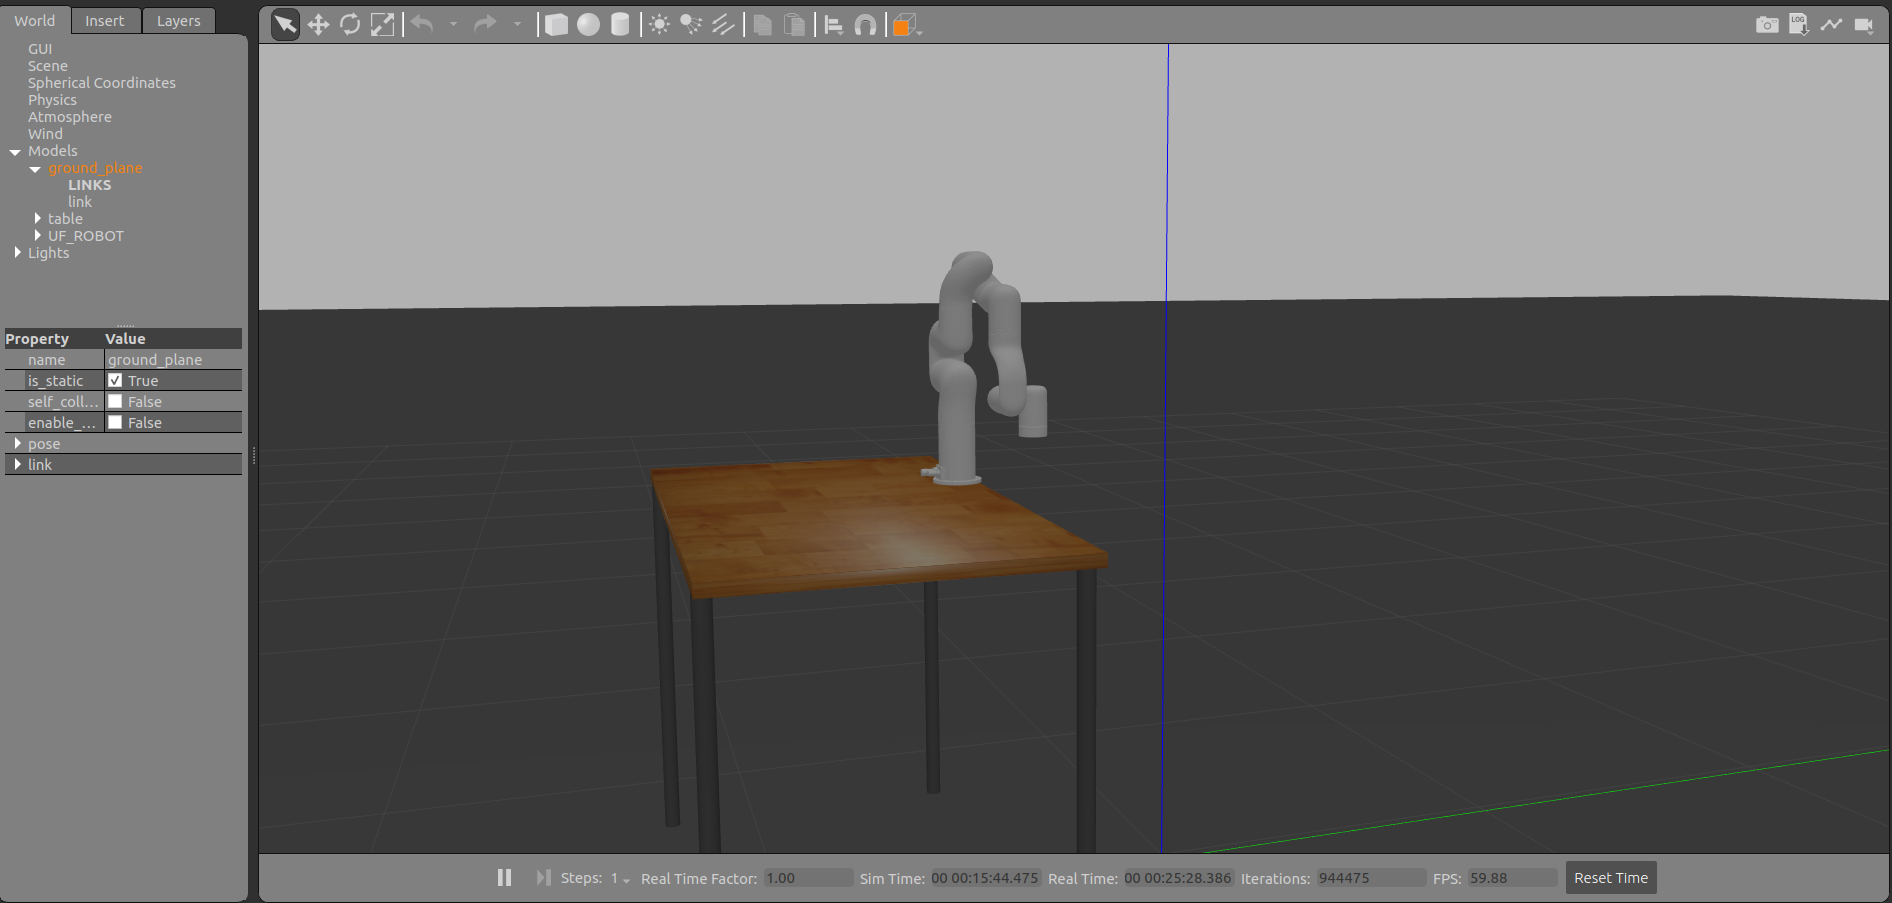
\includegraphics[width=0.48\textwidth]{images/home.png}
    \caption{Simulación del robot en Gazebo sobre una mesa de trabajo.}
    \label{fig:gazebo_home}
\end{figure}

Los movimientos se realizaron enviando metas articuladas mediante un script en Python que utiliza la acción \texttt{FollowJointTrajectory}. El comportamiento fue coherente con las limitaciones cinemáticas del brazo y la configuración del modelo URDF.

\section{Generación heurística de una sentadilla}

Para emular una sentadilla con el brazo robótico, se diseñó una secuencia de configuraciones articulares basadas en un análisis heurístico. Este tipo de movimiento fue seleccionado por su naturaleza compacta, repetitiva y biomecánicamente coherente, lo cual permite validar tanto la precisión como la continuidad de la trayectoria generada.

Las configuraciones articulares fueron ajustadas mediante prueba y error, observando visualmente la evolución del efector final en el entorno simulado de Gazebo. Se buscó que el efector descendiera de forma controlada y simétrica, evitando colisiones con la mesa.

\subsubsection*{Implementación de la secuencia}

La secuencia fue implementada con un script en Python que publica trayectorias articuladas al controlador \texttt{xarm6\_traj\_controller}. Se definieron al menos tres poses consecutivas que simulan el descenso y ascenso del efector final, manteniendo la base fija:

\begin{enumerate}
    \item \textbf{Postura inicial:} configuración articulada equivalente a la posición "home".
    \item \textbf{Descenso parcial:} los ángulos del hombro y codo se ajustan para reducir la altura del efector.
    \item \textbf{Descenso completo:} se maximiza el efecto de la articulación 5 para llevar el efector al punto más bajo.
    \item \textbf{Regreso a postura inicial.}
\end{enumerate}

\subsubsection*{Verificación visual}

La Figura~\ref{fig:sentadilla} muestra la postura intermedia durante la ejecución de la sentadilla. Esta fue capturada en Gazebo y confirma que el efector sigue una trayectoria vertical descendente. Se verificó además que el controlador interpolara correctamente entre las poses sin generar oscilaciones ni comportamientos inesperados.

\begin{figure}[H]
    \centering
    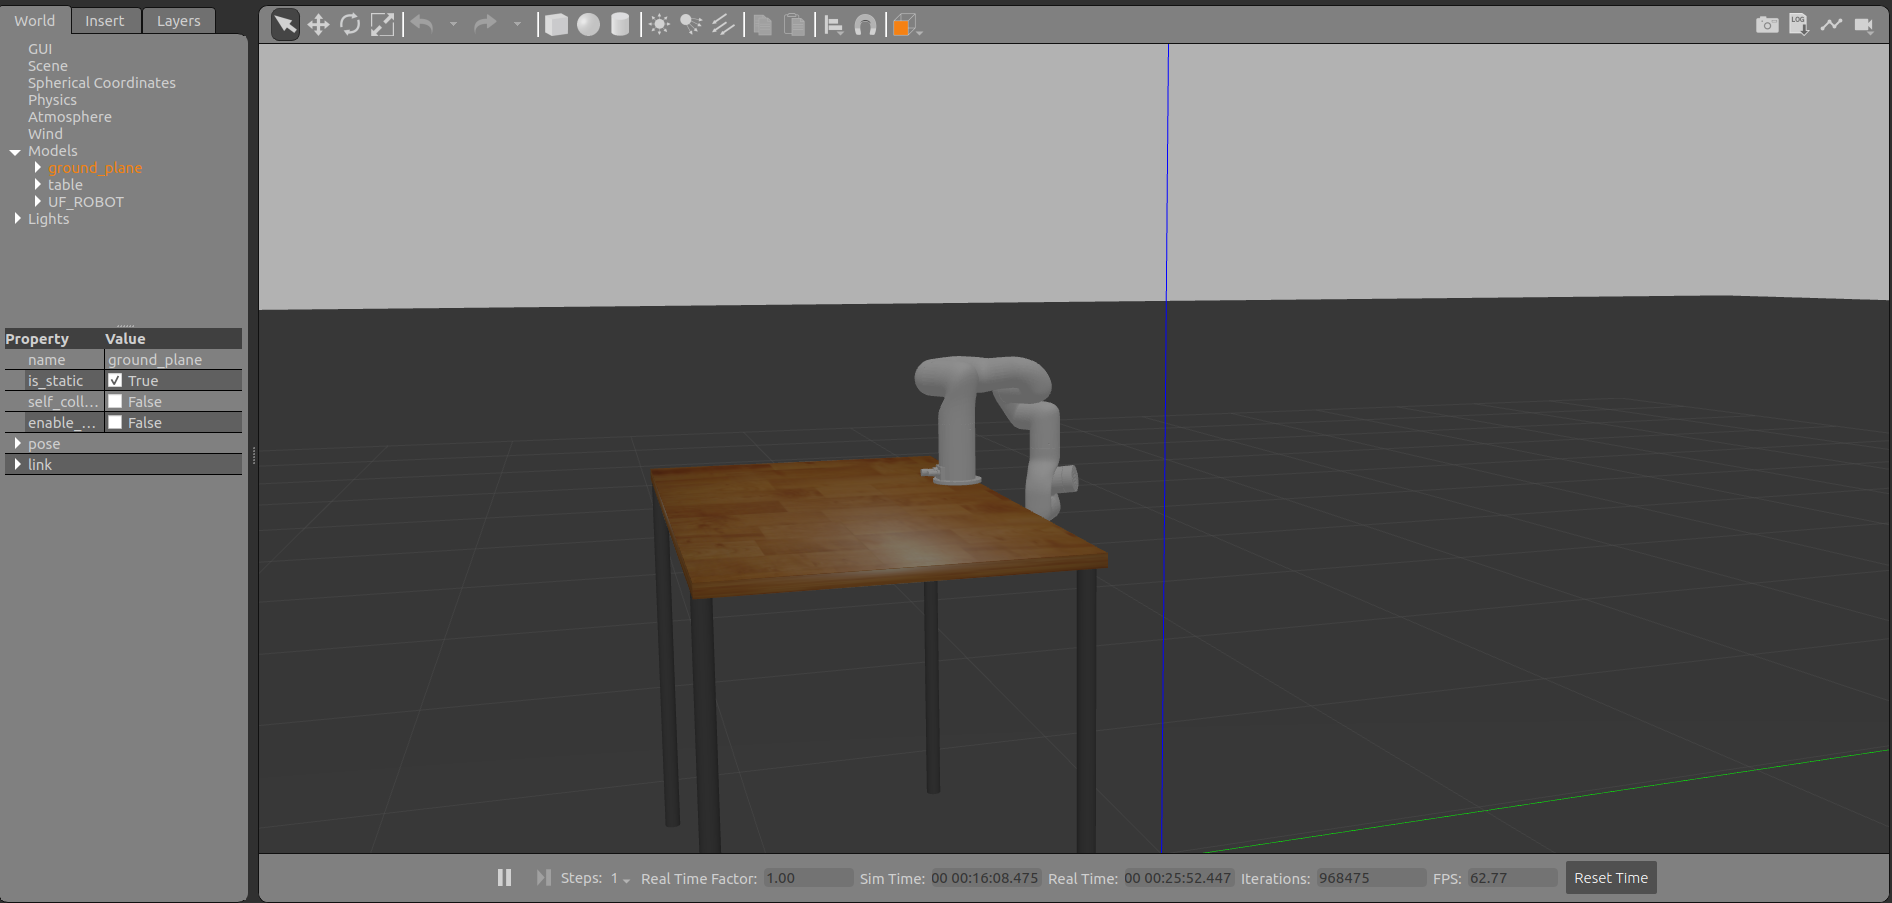
\includegraphics[width=0.48\textwidth]{images/movimiento.png}
    \caption{Movimiento intermedio del robot durante la sentadilla simulada.}
    \label{fig:sentadilla}
\end{figure}

\begin{figure}[H]
    \centering
    \href{https://youtu.be/BZCWY3WiM1Q}{%
        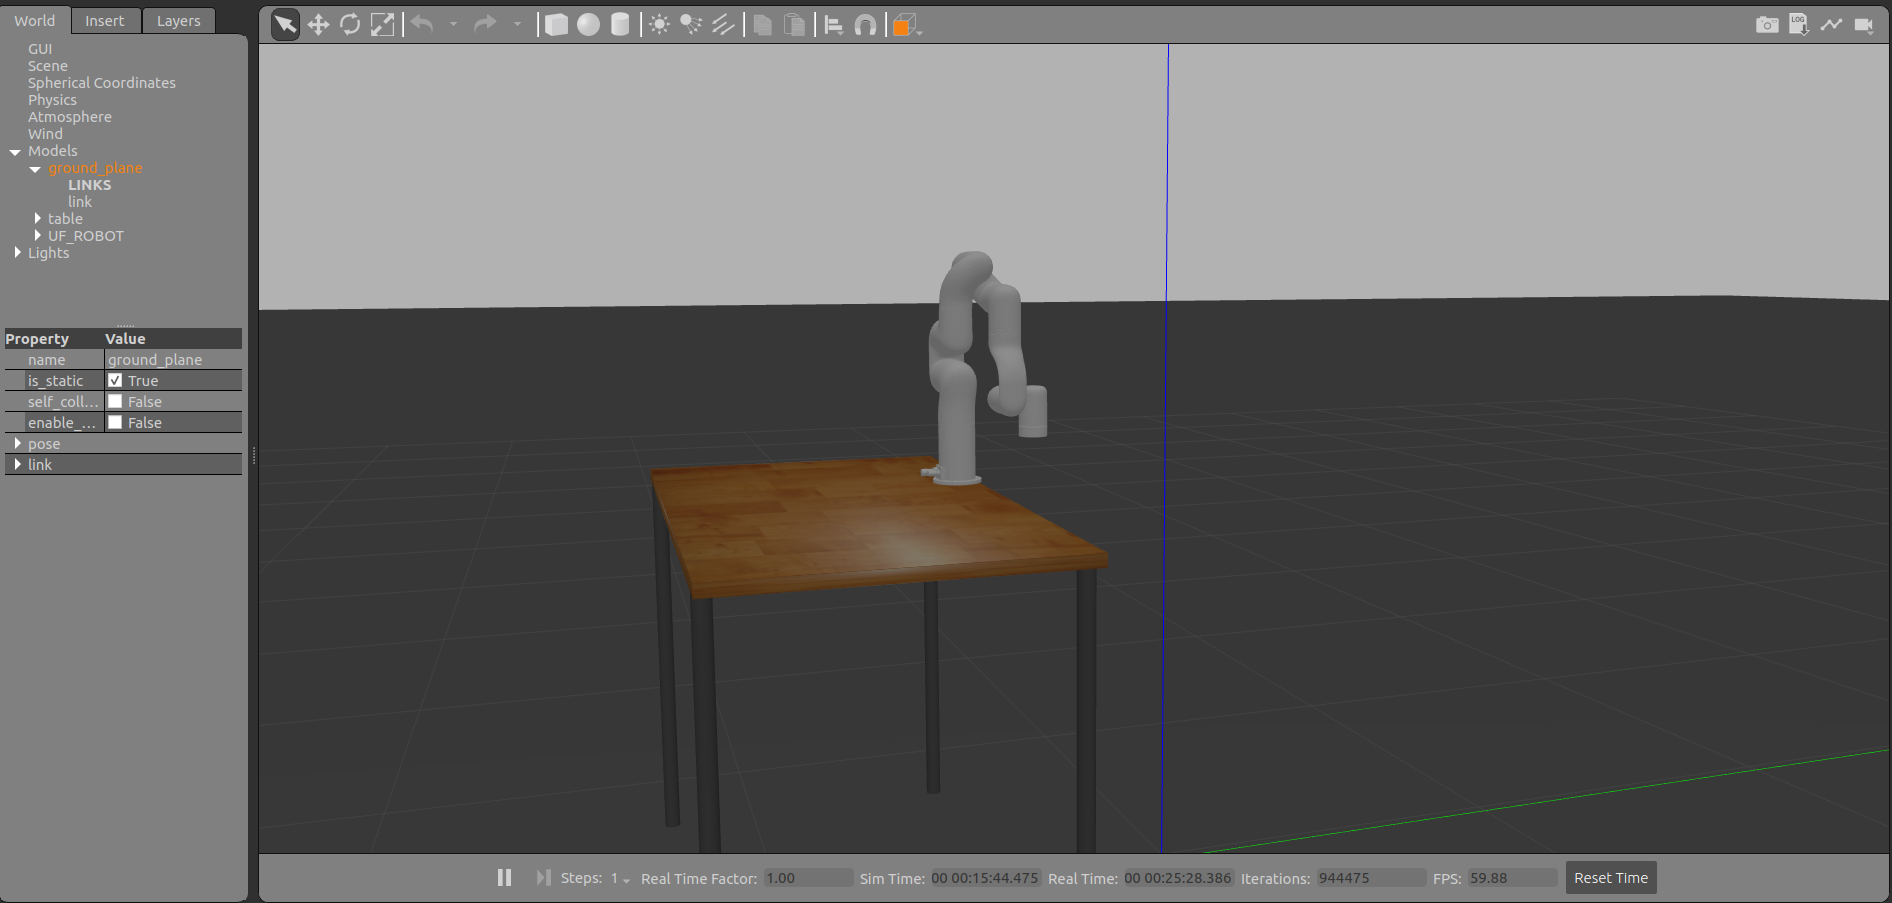
\includegraphics[width=0.490\textwidth]{images/home.png}
    }
    \caption{Demostración en video del sistema funcionando.}
    \label{fig:video_demo}
\end{figure}

\section{Conclusión}

En este trabajo se integraron múltiples herramientas del ecosistema ROS~2 para modelar, visualizar y controlar un brazo robótico en entornos simulados con RViz y Gazebo. Se construyó la tabla de Denavit-Hartenberg para una sección del robot, permitiendo comprender su cadena cinemática. Posteriormente, se validó visualmente la posición del efector final mediante la publicación de un marcador esférico en RViz, comparando su ubicación con la transformada TF publicada por el modelo.

Además, se logró simular el robot en Gazebo con controladores configurados, empleando el stack de \texttt{ros2\_control} para permitir la ejecución de comandos articulados. Finalmente, se diseñó una secuencia de movimientos que emulan una sentadilla, demostrando la capacidad del robot para ejecutar trayectorias complejas y articuladas con estabilidad.

Este proyecto sentó las bases para futuras tareas de control más avanzadas como seguimiento de trayectorias con realimentación sensorial o aprendizaje de movimientos por demostración.

\begin{thebibliography}{00}
\bibitem{xarm_doc} UFACTORY, “xArm6 Technical Manual,” [Online]. Available: \url{https://www.ufactory.cc/download/xArm6}.
\bibitem{ros2_control} ROS 2 Control, “ros2\_control Documentation,” [Online]. Available: \url{https://control.ros.org/}.
\bibitem{gazebo_ros_pkgs} Open Source Robotics Foundation, “gazebo\_ros\_pkgs,” [Online]. Available: \url{http://gazebosim.org/tutorials?tut=ros_overview}.
\bibitem{tf2} ROS 2 TF2 Library, “tf2 Tutorials,” [Online]. Available: \url{https://docs.ros.org/en/rolling/Tutorials/Intermediate/Tf2/Tf2-Main.html}.
\bibitem{denavit} J. Denavit and R.S. Hartenberg, “A kinematic notation for lower-pair mechanisms based on matrices,” ASME Journal of Applied Mechanics, vol. 22, pp. 215–221, 1955.
\bibitem{rviz} ROS, “RViz - ROS Wiki,” [Online]. Available: \url{http://wiki.ros.org/rviz}.
\end{thebibliography}

\end{document}
